\documentclass[11pt]{article}
\usepackage[letterpaper,margin=1in,headheight=15pt]{geometry}
\usepackage{amsmath,amssymb,amsthm,mathtools}
\usepackage{fontspec,unicode-math}
\setmainfont{TeX Gyre Pagella}
\setsansfont{TeX Gyre Heros}[Scale=MatchLowercase]
\setmathfont{TeX Gyre Pagella Math}
\usepackage{microtype,xcolor,booktabs,enumitem,fancyhdr,titlesec,xurl,array,tabularx,tikz}
\usetikzlibrary{arrows.meta,positioning}
\definecolor{Ink}{HTML}{17384B}\definecolor{Link}{HTML}{176078}\definecolor{Accent}{HTML}{7A3E14}
\usepackage[colorlinks=true,linkcolor=Link,urlcolor=Link,citecolor=Link,bookmarksnumbered=true]{hyperref}
\usepackage{bookmark}
\setlength{\parindent}{0pt}\setlength{\parskip}{4.5pt plus 1pt}
\setlength{\emergencystretch}{2em}\setlength{\tabcolsep}{4pt}
\setlist{topsep=3pt,itemsep=2pt,parsep=1pt,leftmargin=*}
\setcounter{tocdepth}{2}
\titleformat{\section}{\Large\bfseries\color{Ink}}{\thesection}{0.7em}{}
\titleformat{\subsection}{\large\bfseries\color{Ink}}{\thesubsection}{0.6em}{}
\titleformat{\subsubsection}{\normalsize\bfseries\color{Ink}}{\thesubsubsection}{0.6em}{}
\titlespacing*{\section}{0pt}{16pt}{7pt}
\titlespacing*{\subsection}{0pt}{12pt}{4pt}
\pagestyle{fancy}\fancyhf{}
\fancyhead[L]{\small\sffamily Classical simulation of quantum queries}
\fancyhead[R]{\small\sffamily AA, Gibbs histories, and certified randomness}
\fancyfoot[C]{\small\thepage}\renewcommand{\headrulewidth}{0.3pt}
\newtheorem{theorem}{Theorem}[section]
\newtheorem{lemma}[theorem]{Lemma}
\newtheorem{proposition}[theorem]{Proposition}
\newtheorem{corollary}[theorem]{Corollary}
\theoremstyle{definition}\newtheorem{definition}[theorem]{Definition}
\newtheorem{example}[theorem]{Example}
\newtheorem{problem}[theorem]{Open problem}
\theoremstyle{remark}\newtheorem{remark}[theorem]{Remark}
\newcommand{\E}{\mathbb E}\newcommand{\Prb}{\mathbb P}
\newcommand{\mc}{\mathcal}\newcommand{\eps}{\varepsilon}
\DeclareMathOperator{\Inf}{Inf}\DeclareMathOperator{\Var}{Var}
\DeclareMathOperator{\TV}{TV}\DeclareMathOperator{\FC}{FC}
\DeclareMathOperator{\poly}{poly}\DeclareMathOperator{\CAdv}{CAdv}
\newcommand{\tagX}[1]{\stepcounter{equation}\tag{#1}}
\newcommand{\dd}{\mathrm d}\newcommand{\set}[1]{\left\{#1\right\}}
\title{\textbf{Classical Simulation of Quantum Queries}\\[5pt]
{\Large Aaronson--Ambainis, Gibbs Histories, and Certified Randomness}}
\author{AA research team}
\date{November 2026}

\begin{document}
\maketitle
\thispagestyle{fancy}
\begin{abstract}
\noindent
We present two query-bounded classical reductions, and a characterization of when classical simulation survives a change of input law, arising from the Aaronson--Ambainis (AA) connection between quantum acceptance probabilities and bounded polynomials. After an expository account of the influential-variable proof and of scalar simulation and bit fixing, we first extend mean quantum-query simulation beyond product input laws. For every finite-parameter classical Gibbs Hamiltonian with weighted interaction strength $\omega\leq1/8$, we give a deterministic classical simulator for any $T$-query quantum acceptance function, using $O(T^{18}e^{-28})$ physical spin queries and achieving mean absolute error at most $e$ under the Gibbs law. Exact sparse update maps, stationary histories, lazy posterior sampling, a product-alphabet adversary argument, and a recursive hybrid estimate form its proof; arbitrary fields, dimension, interaction arity, and positive-probability pinnings are admitted. Second, we give a direct hashing reduction from a heavy valid quantum output to a classical search solver using scalar AA estimates. This yields accepted-output min-entropy bounds, a modular alternative to Yamakawa--Zhandry's threshold/frequency extraction, sparse-output sampling, and, for the unchanged Yamakawa--Zhandry relation, a retuned classical soundness analysis giving entropy $\Omega(\lambda/\log\lambda)$ under the stated acceptance and exceptional-oracle hypotheses. A separate honest-preparation refinement uses $n_{\rm c}$ queries in one parallel layer, where $n_{\rm c}$ is the YZ code length, not the number of Gibbs spins. We compare all reductions with prior work and identify their limitations. The Gibbs result is a mean query-simulation theorem, not polynomial-influence AA for Gibbs measures; the entropy result does not use the Gibbs theorem; and all running-time, quantum-side-information, and unqualified optimality claims are outside our scope. Third, for arbitrary input laws on the cube we prove that classical acceptance simulation fails exactly when there are polynomially weighted \emph{hard sectors}, on which a quantum acceptance function has constant variance but is nearly uncorrelated with every shallow decision tree. We show that a dimension-uniform R\'enyi bound of order $\alpha>1$ transfers simulation while order one does not, give explicit failing laws from Simon's problem, forrelation and the character code, prove that failure forces a hidden (label, transcript) explanation but not a label-only one, and obtain hereditary simulation for Ising laws with $\|K\|_{\rm op}\le1/8$ and bounded Frobenius norm.
\end{abstract}
\tableofcontents
\clearpage

\section{Introduction}\label{sec:introduction}
Quantum query algorithms draw a sharp line between unstructured decision problems and structured search problems. For a total Boolean function, quantum and deterministic query complexities are polynomially related. Relative to a random oracle, however, quantum search can be exponentially easier than classical search. The Aaronson--Ambainis (AA) influential-variable theorem explains a corresponding limitation for decision problems: a bounded degree-$d$ polynomial with substantial variance has an influential coordinate, with a bound polynomial in variance and inverse degree. Its original quantum-query acceptance consequence supplies deterministic classical estimates on most uniformly random inputs \cite{AA14,Tur26,BDST26}.

The three research branches in this paper ask different questions about that classical-simulation interface.
\begin{itemize}
\item \textbf{Can the input law be correlated?} We represent high-temperature Gibbs configurations by exact histories on an independent tape of signed-parity or constant update maps. Quantum queries can then be answered first on this product source and transferred back to physical spins with explicit error and work bounds.
\item \textbf{What useful output information can scalar simulation recover?} Even when classical search is exponentially hard, scalar AA estimates can reconstruct a valid output whenever one has nonnegligible probability. Hashing makes this extraction explicit and turns a low-entropy hypothesis into a classical-search contradiction.
\item \textbf{What exactly fails when simulation fails?} For an arbitrary input law, failure of simulation is characterized by hard sectors, which yields sharp transfer criteria, explicit failing laws, and a precise test of the ``hidden phase label'' intuition (Section~\ref{sec:distributional}).
\end{itemize}
The first two branches meet methodologically but do not imply one another. No theorem below uses the Gibbs simulator to prove certified randomness, and no Gibbs lemma depends on hashing.

\begin{center}
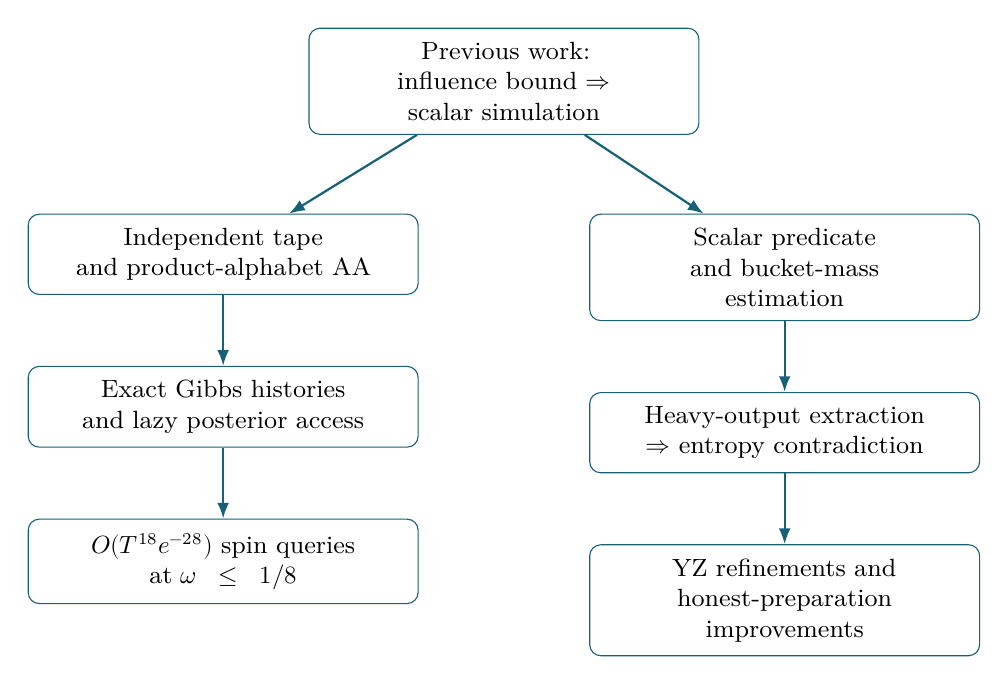
\begin{tikzpicture}[
node distance=9mm and 11mm,
box/.style={draw=Link,rounded corners,align=center,inner sep=5pt,text width=46mm,font=\small},
arr/.style={-{Latex[length=2mm]},draw=Link,thick}]
\node[box] (aa) {Previous work:\\influence bound $\Rightarrow$ scalar simulation};
\node[box,below left=10mm and -14mm of aa] (gibbs) {Independent tape\\and product-alphabet AA};
\node[box,below right=10mm and -14mm of aa] (hash) {Scalar predicate and bucket-mass\\estimation};
\node[box,below=of gibbs] (hist) {Exact Gibbs histories\\and lazy posterior access};
\node[box,below=of hash] (entropy) {Heavy-output extraction\\$\Rightarrow$ entropy contradiction};
\node[box,below=of hist] (gq) {$O(T^{18}e^{-28})$ spin queries\\at $\omega\leq1/8$};
\node[box,below=of entropy] (yz) {YZ refinements and\\honest-preparation improvements};
\draw[arr] (aa)--(gibbs); \draw[arr] (aa)--(hash);
\draw[arr] (gibbs)--(hist); \draw[arr] (hash)--(entropy);
\draw[arr] (hist)--(gq); \draw[arr] (entropy)--(yz);
\end{tikzpicture}
\end{center}

\subsection*{Contributions and claim status}
Sections~\ref{sec:background} reviews previous work. It includes a guided sketch of the influential-variable proof, rather than presenting that proof as an event contribution. Turturean's original manuscript reports stronger exponents than the BDST exposition used for our displayed scalar bound \cite{Tur26,BDST26}. Turturean also states that Theorem~1.1 and Corollary~1.2 of that work were checked by the Lean kernel. \textbf{No analogous formalization of the assembled results in this paper is asserted.}

Our Gibbs contribution is stated precisely in Theorem~\ref{main}. Its constant is dimension-free under $\omega\leq1/8$ and computation is free. It is neither efficient sampling, a full-Dobrushin theorem, nor a polynomial-influence theorem for bounded polynomials on Gibbs measures. Product-alphabet influences below are coordinate-resampling influences, distinct from uniform Boolean flip influence.

Section~\ref{sec:distributional} reports Ian Loam's work on general input laws. Its central result, Theorem~\ref{dist:equivalence}, characterizes failure of acceptance simulation by hard sectors and uses no imported theorem. Its positive results rely on the product-alphabet simulator, and through it on inequality (BC) of \cite{HMP26}. It extends the product and slice transfers of Girish--Mittal--Nehoran--Raz \cite{GMNR26} to arbitrary laws. Its influence-form remark has weaker exponents than \cite{Tur26} and is not claimed as an improvement. Those notes were drafted with the AI assistant Astra and checked by their author lemma by lemma, and the section was condensed with Claude (Anthropic).

Our certified-randomness contributions are Theorems~\ref{heavy}--\ref{sparse}. Yamakawa--Zhandry (YZ) proved the AA-to-entropy route \textbf{conditionally on the AA simulation conjecture} \cite[Theorem 8.4 and Conjecture 8.1]{YZ24}; the 2026 influence proofs supply that hypothesis, which is now a theorem. Our extraction is an alternative factorization through explicit bucket predicates, with explicit exponents, and our coding and honest-preparation refinements are separate inputs. It is not the first use of AA in this setting. Independent work has proved security of the same YZ protocol unconditionally against $o(\log\lambda)$ adaptive quantum queries and against subexponentially many adaptive quantum queries \cite{KRT26,CKMRSST26}. We do not claim to remove an assumption that those works did not already avoid, nor a uniform improvement over their adversary classes. Quantitative comparisons are upper-bound comparisons under one common scalar simulation bound, not optimality claims. Additional comparison and sampling analyses appear in the appendices to keep the main line readable.

\input{results/unified_aa_sections/background}
\input{results/unified_aa_sections/gibbs_intro}
\input{results/unified_aa_sections/gibbs_core}
% Distributional AA: hard sectors, transfer, phase labels, spectral high temperature.
% Condensed from notes/ian/ (Ian Loam, commits of 2026-11-14 and 2026-11-15).
% Every statement below was compared with the cited note file; file names are
% given so that each full proof can be checked there.
% TODO(integration): once gibbs_core.tex is recovered, replace the hard-coded
% "Lemma 3.8 / Section 3.6" (numbering of the 36-page PDF) by \ref to its label.
% Checked against the PDF: Lemma 3.8 is the O(T^6 e^{-15}) product-alphabet
% simulator (importing [HMP26, Lemma 4, eq. (4)]), and for pair interactions the
% weighted interaction strength of Theorem~\ref{main} is beta*max_i sum_j |J_ij|.
\providecommand{\Cov}{\operatorname{Cov}}
\providecommand{\R}{\mathbb R}
\providecommand{\Hard}{\operatorname{Hard}}

\section{When does acceptance simulation survive a change of input law?}\label{sec:distributional}

\paragraph{Contributor and status.}
This section reports work of Ian Loam during the event (\texttt{notes/ian/},
files \texttt{01}--\texttt{38}). It follows a research outline Ian wrote by hand
before formalizing anything. The note files were drafted with the AI assistant
Astra and checked by Ian lemma by lemma before inclusion. Claude (Anthropic)
helped condense them into this section, and each statement below was compared
with its note file. Unless marked otherwise, every result is \emph{proved}. The
only import is the product-alphabet simulator of
Theorem~\ref{dist:product-sim}, which relies on inequality~(BC) of
Huffstutler--Miloschewsky--Podder~\cite{HMP26}. Where other literature is used,
it is named at the point of use. No result in this section is machine-checked.

\paragraph{Question and relation to prior work.}
Girish, Mittal, Nehoran and Raz~\cite{GMNR26} showed that polynomial-overhead
classical simulation of quantum queries, and the influence form of AA, carry
over from the uniform cube to biased product laws and to Hamming slices. The
Gibbs theorem of this paper (Theorem~\ref{main}) extends acceptance simulation to
one class of high-temperature Gibbs laws. This section asks the general
question: \emph{for which input laws does acceptance simulation hold, and what
exactly goes wrong when it fails?} We give
(i)~an exact characterization of failure by \emph{hard sectors}
(Theorem~\ref{dist:equivalence});
(ii)~sharp transfer criteria between laws, with Rényi order one as the precise
threshold (Propositions~\ref{dist:lp-transfer}--\ref{dist:kl});
(iii)~explicit failing families built from Simon's problem, forrelation and the
character code (Theorem~\ref{dist:failures});
(iv)~a phase-label theorem: failure forces a \emph{hidden} latent explanation,
but not a label-only one (Theorem~\ref{dist:phase-converse},
Proposition~\ref{dist:label-only-fails}); and
(v)~positive results for Ising laws with operator-norm interaction bounds,
which reach a regime the weighted-interaction hypothesis does not
(Theorems~\ref{dist:one-query} and~\ref{dist:frobenius}).
Items (i)--(iv) concern arbitrary laws on the cube. Item~(v) complements the
Gibbs theorem of this paper, which it neither implies nor uses.

\subsection{Setting}\label{dist:setting}
Let \(\Omega_n=\{-1,1\}^n\). We write \(\mc Q_{n,T}\) for the acceptance
functions \(Q:\Omega_n\to[0,1]\) of quantum algorithms that make at most \(T\)
coordinate queries. Let \(\mc D_t\) (resp.\ \(\mc F_t\)) be the deterministic
adaptive coordinate decision trees of worst-case depth at most \(t\) with leaf
outputs in \([0,1]\) (resp.\ \([-1,1]\)). Computation is free. For a law \(\mu\)
on \(\Omega_n\) put
\[
 \ell_\mu(t,Q)=\min_{D\in\mc D_t}\E_\mu|D-Q| .
\]
This minimum exists, and it is nonincreasing in \(t\). For
\(f:\Omega_n\to\R\) write \(D_if(x)=(f(x_{-i},1)-f(x_{-i},-1))/2\) and
\(I_i^\mu(f)=\E_\mu(D_if)^2\).

\begin{definition}[Full AA]\label{dist:full-aa}
A family \(\boldsymbol\mu=(\mu_n)_{n\ge1}\) has \emph{full AA} if there are
constants \(A_0,B_0\ge1\) such that
\(\ell_{\mu_n}(\lceil A_0(T+\eps^{-1})^{B_0}\rceil,Q)\le\eps\) for all
\(n,T\ge1\), all \(\eps\in(0,1)\) and all \(Q\in\mc Q_{n,T}\). The constants may
depend on the family, and they are fixed before \(n,T,\eps,Q\). The family has
\emph{hereditary} full AA if the same constants serve every positive-probability
pinning of every \(\mu_n\).
\end{definition}
Full AA is the mean-absolute-error, deterministic, dimension-free notion of
simulation used by the Gibbs theorem. For the uniform law it is the
scalar-simulation consequence of AA.

\begin{definition}[Hard laws and sectors]\label{dist:hard}
Let \(Q:\Omega_n\to[0,1]\) and \(0<\gamma<a\le1/4\). A law \(\nu\) satisfies
\(\Hard(Q,\nu;t,a,\gamma)\) if
\[
 \Var_\nu Q\ge a
 \qquad\text{and}\qquad
 |\Cov_\nu(Q,F)|\le\gamma\ \text{ for every }F\in\mc F_t .
\]
A \emph{smooth sector} of \(\mu\) of weight \(w\in(0,1]\) is a hard law \(\nu\)
with \(w\nu\le\mu\) pointwise. A \emph{set sector} of weight \(w\) is a set
\(H\) with \(\mu(H)\ge w\) whose conditional law \(\mu(\cdot\mid H)\) is hard.
Every set sector is a smooth sector of the same weight.
\end{definition}
In words: on a hard sector, \(Q\) has constant spread but is almost
uncorrelated with every shallow classical test.

\begin{theorem}[Product-alphabet simulator; Section~3.6, Lemma~3.8]\label{dist:product-sim}
For every finite product measure on finite alphabets and every \(T\)-query
acceptance function \(Q\), there is a deterministic classical symbol-query
simulator with mean error at most \(e\) using \(O(T^6e^{-15})\) queries. The
absolute implied constant does not depend on alphabet sizes, biases or the
number of coordinates.
\end{theorem}
This restates the product-alphabet lemma proved in the Gibbs part of this
paper (Section~3.6, Lemma~3.8; also
\path{notes/foundations/product_alphabets.tex}). It is not part of Ian's work.
Every positive statement below uses it as the uniform-input ingredient. Its only
external input is the counting inequality~(BC) of~\cite{HMP26}.

\subsection{Hard sectors characterize the failure of full AA}\label{dist:sectors}

\begin{proposition}[Forward bound; \texttt{ian/13}]\label{dist:forward}
If \(\nu\) is a smooth sector of \(\mu\) of weight \(w\) and
\(\Hard(Q,\nu;t,a,\gamma)\) holds, then \(\ell_\mu(t,Q)\ge w(a-\gamma)\).
\end{proposition}
\begin{proof}
Let \(D\in\mc D_t\) and \(m=\E_\nu Q\). Since \(2D-1\in\mc F_t\), hardness gives
\(\Cov_\nu(Q,D)\le\gamma/2\). Hence
\(\E_\nu(Q-D)^2=\Var_\nu Q+\E_\nu(D-m)^2-2\Cov_\nu(Q,D)\ge a-\gamma\). On
\([0,1]\) we have \(|Q-D|\ge(Q-D)^2\), and \(\mu\ge w\nu\), so
\(\E_\mu|Q-D|\ge w(a-\gamma)\).
\end{proof}
The converse is the substance of this subsection. It uses no quantum property
of \(Q\).

\begin{theorem}[One calibrated predictor; \texttt{ian/13}]\label{dist:regularity}
Let \(\mu\) be a law on \(\Omega_n\), \(Q:\Omega_n\to[0,1]\), \(t\ge1\),
\(0<\gamma<a\le1/4\), \(0<w\le1\), \(M=\lceil1/\gamma\rceil\) and \(K\ge1\). At
least one of the following holds:
\begin{enumerate}
\item there is \(H\subseteq\Omega_n\) with \(\mu(H)\ge w\) and
\(\Hard(Q,\mu(\cdot\mid H);t,a,\gamma)\); moreover, \(H=g^{-1}(I)\) for an
interval \(I\) and a function \(g\) computed by a tree of depth below \(Kt\);
\item \(\ell_\mu(Kt,Q)\le\sqrt a+\tfrac12\bigl(Mw+1/(K\gamma^2)\bigr)\).
\end{enumerate}
\end{theorem}
\begin{proof}
Let \(R_j=\min_{D\in\mc D_{jt}}\E_\mu(Q-D)^2\). This is nonincreasing, and
\(R_0=\Var_\mu Q\le1/4\). Hence some \(k<K\) has \(R_k-R_{k+1}\le1/(4K)\). Let
\(g\) attain \(R_k\), and let \(\mc A\) be its leaf partition. Optimal leaves
are conditional means, so \(g=\E_\mu[Q\mid\mc A]\), and
\(\E_\mu[(Q-g)\mathbf 1_B]=0\) for every \(\mc A\)-measurable \(B\).

Cut \([0,1]\) into \(M\) intervals \(I_j\) of length \(1/M\) with midpoints
\(c_j\). Let \(H_j=g^{-1}(I_j)\), \(p_j=\mu(H_j)\) and
\(\nu_j=\mu(\cdot\mid H_j)\). Call a bin \emph{bad} if some
\(F_j\in\mc F_t\) has \(\Cov_{\nu_j}(Q,F_j)>\gamma\). On a bad bin,
\(|g-c_j|\le\gamma/2\) gives \(|\Cov_{\nu_j}(g,F_j)|\le\gamma/2\), so
\(\E_{\nu_j}[(Q-g)F_j]>\gamma/2\). Let \(p\) be the bad mass and
\(Z=\sum_{j\text{ bad}}\mathbf 1_{H_j}F_j\). Running \(F_j\) after the tree for
\(g\) gives depth at most \((k+1)t\), and a partition \(\mc A'\) refining \(\mc A\)
with \(Z\) measurable. For \(g'=\E_\mu[Q\mid\mc A']\), Pythagoras and
Cauchy--Schwarz give
\[
 \tfrac1{4K}\ge R_k-R_{k+1}\ge\E_\mu(g'-g)^2
 \ge\frac{(\E_\mu[(Q-g)Z])^2}{\E_\mu Z^2}>\frac{p\gamma^2}{4},
\]
so \(p\le1/(K\gamma^2)\). Now suppose item~1 fails. Then every bin with
\(\Var_{\nu_j}Q\ge a\) is bad or has mass below \(w\). The tree that outputs
\(m_j=\E_{\nu_j}Q\) on \(H_j\) has loss below \(\sqrt a\) on the other bins, by
Cauchy--Schwarz, and at most \(1/2\) on these. This gives item~2.
\end{proof}
The argument is an energy-increment (multicalibration) argument in the spirit
of~\cite{TTV09,HKRR18,CDV24}. None of these works is used in the proof.

\begin{corollary}[Explicit extraction; \texttt{ian/13}]\label{dist:extraction}
Let \(0<\eps<1/8\), \(0<\eta\le1/4\) and
\(L=\lceil32\eps^{-5}\eta^{-2}\rceil t\). Suppose \(\ell_\mu(L,Q)>\eps\). Then
there is a set \(H\), decided by a tree of depth below \(L\), with
\[
 \mu(H)\ge\eta\eps^3/16
 \qquad\text{and}\qquad
 \Hard\bigl(Q,\mu(\cdot\mid H);t,\eps^2/4,\eta\eps^2/4\bigr).
\]
No atom-size hypothesis on \(\mu\) is needed.
\end{corollary}
\begin{proof}
Apply Theorem~\ref{dist:regularity} with \(a=\eps^2/4\), \(\gamma=\eta a\),
\(w=\eps/(2M)\ge\eta\eps^3/16\) and \(K=\lceil2/(\eps\gamma^2)\rceil\). Then
item~2 would give loss at most \(\eps/2+\eps/4+\eps/4=\eps\), which is excluded.
\end{proof}

\begin{theorem}[Failure of full AA \(\iff\) polynomially weighted hard sectors; \texttt{ian/13}]\label{dist:equivalence}
For every family \(\boldsymbol\mu\) the following are equivalent:
\begin{enumerate}
\item full AA fails;
\item for every \(A,B\ge1\) there are \(n,T\ge1\), \(r>8\),
\(Q\in\mc Q_{n,T}\) and \(H\subseteq\Omega_n\) such that, with
\(t=\lceil A(T+r)^B\rceil+1\),
\[
 \mu_n(H)\ge\frac1{64r^3}
 \qquad\text{and}\qquad
 \Hard\Bigl(Q,\mu_n(\cdot\mid H);t,\frac1{4r^2},\frac1{16r^2}\Bigr);
\]
\item the same holds with a smooth sector \(\nu\le64r^3\mu_n\) in place of
\(\mu_n(\cdot\mid H)\).
\end{enumerate}
\end{theorem}
\begin{proof}[Proof sketch; full constants in \texttt{ian/13}]
(1)\(\Rightarrow\)(2): a short reduction allows \(\eps=1/r<1/8\). Apply full-AA
failure with budget \((1026A,B+5)\), which dominates
\(L=\lceil512r^5\rceil t\), and then apply Corollary~\ref{dist:extraction} with
\(\eta=1/4\). (2)\(\Rightarrow\)(3) holds because
\(\mu_n(\cdot\mid H)\le\mu_n/\mu_n(H)\). For (3)\(\Rightarrow\)(1), suppose full
AA holds with constants \((A_0,B_0)\). Then
Proposition~\ref{dist:forward} gives \(\ell_{\mu_n}(t,Q)\ge3/(1024r^5)\). The
witness for \((A,B)=(2^{10B_0}A_0,5B_0)\) has \(t\) exceeding the depth at which
full AA forces loss at most half of that.
\end{proof}
The weight and dispersion are fixed polynomials in \(r\), independent of the
budget constants. Thus failure of full AA is witnessed by a \emph{single}
explicit kind of object, and that object is a property of the input law alone.
The common-exponent form (``H1'') remains open, with one exponent \(C\) in place
of the three exponents \(3,2,2\) in \(r\). The notes prove that no extraction
whose depth depends only on \((\eps,\eta,t)\) can guarantee dispersion above
\(4\eps^2\) (\texttt{ian/14}).

\subsection{Transfer between laws, and its limit}\label{dist:transfer}
\begin{proposition}[Density transfer; \texttt{ian/16}]\label{dist:lp-transfer}
Let \(\mu,\nu\) be laws on \(\Omega_n\), let \(\rho=\dd\nu/\dd\mu\), and let
\(p\in(1,\infty]\) with conjugate exponent \(q\). If
\(\|\rho\|_{L^p(\mu)}\le K\), then
\(\ell_\nu(t,Q)\le K\,\ell_\mu(t,Q)^{1/q}\) for every \(t\) and every \(Q\). In
particular:
\begin{enumerate}
\item a dimension-uniform bound on the Rényi divergence \(D_\alpha(\nu_n\|\mu_n)\)
for one fixed \(\alpha>1\) transfers full AA from \(\boldsymbol\mu\) to
\(\boldsymbol\nu\);
\item for \(\mu_n\propto e^{-V_n}\pi_n\) with \(\pi_n\) a product law and
\(W_n=\max V_n-\min V_n\), every \(Q\in\mc Q_{n,T}\) has a deterministic tree of
depth \(O(T^6e^{15W_n}\eps^{-15})\) with \(\E_{\mu_n}|D-Q|\le\eps\). Hence
\(\sup_nW_n<\infty\) implies full AA.
\end{enumerate}
\end{proposition}
\begin{proof}
For \(A=|D-Q|\in[0,1]\), Hölder's inequality and \(A^q\le A\) give
\(\E_\nu A\le K(\E_\mu A)^{1/q}\). For item~1, use
\(\|\rho\|_{L^\alpha}=e^{(1-1/\alpha)D_\alpha}\). For item~2, use
\(\dd\mu_n/\dd\pi_n=e^{-V_n}/\E_{\pi_n}e^{-V_n}\le e^{W_n}\) and apply
Theorem~\ref{dist:product-sim} at error \(\eps e^{-W_n}\).
\end{proof}

\begin{proposition}[Rényi order one is the threshold; \texttt{ian/16}]\label{dist:kl}
There are families with \(D(\nu_n\|\mu_n)\le1\) for every \(n\) such that
\(\boldsymbol\mu\) has full AA and \(\boldsymbol\nu\) does not. For each fixed
\(\alpha>1\), \(D_\alpha(\nu_n\|\mu_n)\to\infty\) along these families.
\end{proposition}
\begin{proof}
Let \(m\) be even and \(n=2^m\). Let
\(C_n=\{c_A:A\in\mathbb F_2^m\}\) be the character code, where
\(c_A(i)=(-1)^{A\cdot i}\) for \(i\in\mathbb F_2^m\), and let \(c_0\) be the
all-ones word. Put
\(\mu_n=(1-\tfrac1m)\delta_{c_0}+\tfrac1mU_{C_n}\) and
\(\nu_n=(1-q_m)\delta_{c_0}+q_mU_{C_n}\) with \(q_m=1/\ln m\). On the support of
\(\mu_n\), reading the \(m\) coordinates \(i=e_1,\dots,e_m\) determines the input.
So \(\mu_n\) is simulated exactly at depth \(m\) when \(\eps<1/m\), and by the
constant \(Q(c_0)\) otherwise. The log-sum inequality gives
\(D(\nu_n\|\mu_n)\le q_m\ln m=1\).

Let \(h\) be a bent quadratic on \(\mathbb F_2^m\), and let \(P(c_A)=h(A)\). This
\(P\) is computed by one phase query followed by a Walsh transform
(Bernstein--Vazirani), and \(\ell_{U_{C_n}}(t,P)\ge(1-2^{t-m/2})/2\) for
\(t\le m/2-2\) (team notes, \texttt{obstructions/character\_code}). Hence
\(\ell_{\nu_n}(t,P)\ge3q_m/8\), which defeats every budget
\(A(1+8\ln m)^B\) once \(m\) is large. For the last claim,
\(\E_{\mu_n}\rho^\alpha\ge(1-\tfrac1n)m^{\alpha-1}/(\ln m)^\alpha\to\infty\).
\end{proof}
Together, Propositions~\ref{dist:lp-transfer} and~\ref{dist:kl} identify
exactly which Rényi-divergence bounds preserve full AA: orders \(\alpha>1\) do,
and orders \(\alpha\le1\) do not. In the example the density ratio is only
\(O(\log n)\). Dimension-dependent density bounds therefore do not suffice.

\subsection{Explicit laws without full AA}\label{dist:failures-sec}
\begin{theorem}[Explicit failures; \texttt{ian/17,30,33}]\label{dist:failures}
In each row of Table~\ref{dist:table}, the stated \(Q\in\mc Q_{n,T}\) and law
satisfy \(\Hard(Q,\mu;t,a,\gamma)\) on a sector of weight one. Since \(t\)
outgrows every polynomial in \(T\), any family containing these laws fails full
AA by Proposition~\ref{dist:forward}.
\end{theorem}
\begin{table}[h]
\centering\small
\begin{tabular}{@{}lllllll@{}}
\toprule
Law (sector of weight \(1\)) & \(n\) & \(T\) & hard depth \(t\) & \(a\) & \(\gamma\) & source\\
\midrule
Character code \(U_{C_n}\), \(P(c_A)=h(A)\) & \(2^m\) & \(1\) & \(m/2-2\) & \(3/16\) & \(1/8\) & \texttt{ian/17}\\
Randomly labelled Simon tables, target \(s_1\) & \(m2^m\) & \(m(m+9)\) & \(\lfloor2^{m/2}/32\rfloor\) & \(1/8\) & \(1/64\) & \texttt{ian/30}\\
Sign-rounded forrelation mixture, \(Q=\frac{1+\Phi}2\) & \(2^{m+1}\) & \(1\) & \(\lfloor2^{m/8}\rfloor\) & \(1/64\) & \(1/256\) & \texttt{ian/33}\\
\bottomrule
\end{tabular}
\caption{Hard-sector parameters. The character row needs \(n\ge16\), the Simon
row \(m\ge10\), and the forrelation row \(m\ge96\).}\label{dist:table}
\end{table}
In the Simon law, a uniform nonzero \(s\in\mathbb F_2^m\) and a uniform injection
\(L\) from the pairs \(\{x,x+s\}\) into \(\mathbb F_2^m\) define
\(f(x)=L(\{x,x+s\})\). The input is the bit table of \(f\), with the labels
sampled without replacement. The quantum algorithm is Simon's~\cite{Sim97},
reproved in the note. In the forrelation row, the two truth tables come from
the equal mixture of \((\mathrm{sgn}A,\mathrm{sgn}C)\) and
\((\mathrm{sgn}A,\mathrm{sgn}WA)\) for independent standard Gaussian vectors
\(A,C\) and the normalized Walsh matrix \(W\). These are the two measures of
Aaronson--Ambainis~\cite{AA15}, and
\(\Phi=2^{-3m/2}f^{\mathsf T}(\sqrt{2^m}W)g\). The quantum mechanisms are
standard. The \emph{new} content is the explicit hard-sector constants. The
forrelation depth \(2^{m/8}\) comes from an adaptive hiding lemma proved in the
note, not from the published \(\Omega(\sqrt M/\log M)\) bound, which has no
explicit bias-versus-depth function. The notes also give period-finding and
finite abelian hidden-subgroup sectors for black-box encoded tables
(\texttt{ian/31}). These are not statements about factoring. They also treat
Hadamard-code sectors, whose mechanism is van Dam's~\cite{vD02}
(\texttt{ian/34}).

\subsection{Hidden phase labels}\label{dist:phase}
Physically, one hopes that failure of simulation is ``explained'' by a hidden
macroscopic label, such as a phase, a period or a secret string. The following
results make this precise and set its limits.

\begin{definition}[Admissible decomposition; \texttt{ian/19}]\label{dist:decomp}
Let \(\mc C\) be a class of laws with a common simulation polynomial \(\Psi\):
\(\ell_\lambda(\lceil\Psi(T,\delta^{-1})\rceil,Q)\le\delta\) for all
\(\lambda\in\mc C\), all \(Q\in\mc Q_{N,T}\) and all \(\delta\in(0,1)\). A
\emph{decomposition} of \(\boldsymbol\mu\) is a mixture
\(\mu_N=\int\mu_{N,z}\,\pi_N(\dd z)\) with every \(\mu_{N,z}\in\mc C\). It is
fixed before any acceptance function, accuracy or sector is chosen. Write \(Z\)
for the latent label, and \(\widehat Q=D_Z(X)\) for the output of the
(measurably chosen) component simulator at accuracy \(\delta\).
\end{definition}
For example, \(\mc C\) may consist of the product laws, by
Theorem~\ref{dist:product-sim}.

\begin{theorem}[Phase-label theorem; \texttt{ian/20}]\label{dist:phase-converse}
Suppose full AA fails for \(\boldsymbol\mu\), and fix a decomposition as in
Definition~\ref{dist:decomp}. For every \(\theta_1,\theta_2\ge1\) there are
\(N,T\), \(\eps\in(0,1/8)\), \(Q\in\mc Q_{N,T}\) and \(H\) with
\(\mu_N(H)\ge\eps^3/64\) and \(\Hard(Q,\mu_N(\cdot\mid H);t,a,a/4)\), where
\(a=\eps^2/4\), \(\delta=\eps^7/2^{22}\),
\(s=\lceil\Psi(T,\delta^{-1})\rceil\) and
\(t=\lceil\theta_1(T+\eps^{-1})^{\theta_2}\rceil+s+1\). Let
\(\widetilde Z=(Z,\tau_Z(X))\) consist of the label and the depth-\(s\)
transcript of its component simulator, and let \(M=\E_H[Q\mid\widetilde Z]\).
With \(u=\eps^4/2^{16}\),
\[
 \E_H\Var(Q\mid\widetilde Z)\le u,\qquad
 \Var_HM\ge\Var_HQ-u,\qquad
 |\Cov_H(M,F)|\le\tfrac{a}{4}+\tfrac{a}{64}\quad(F\in\mc F_t).
\]
\end{theorem}
\begin{proof}
Theorem~\ref{dist:equivalence}, applied with budget constants enlarged to absorb
\(s\), gives the sector. Restricting to \(H\) costs the inverse weight, so
\(\E_H|Q-\widehat Q|\le\delta/\mu_N(H)\le u\). Since \(\widehat Q\) is
\(\widetilde Z\)-measurable,
\(\E_H(Q-M)^2\le\E_H(Q-\widehat Q)^2\le u\). The law of total variance gives the
first two claims, and Cauchy--Schwarz gives
\(|\Cov_H(M-Q,F)|\le\sqrt u=a/64\).
\end{proof}
So on a hard sector, the label \emph{together with a shallow transcript}
explains almost all acceptance variance while remaining invisible to shallow
classical tests. The explanation alone does not imply failure, since
\(\widetilde Z=X\) is always an explanation. The theorem is an implication, not
an equivalence. The natural strengthening is false:

\begin{proposition}[Label-only explanation fails; \texttt{ian/19,20,27}]\label{dist:label-only-fails}
\leavevmode
\begin{enumerate}
\item Let \(\mu=U_{C_n}\) and \(Q=P\) as in Table~\ref{dist:table}. Decompose
\(A=\xi+e_\kappa\) with \(\xi\) uniform on \(\mathbb F_2^m\) and \(\kappa\)
uniform on \(\{0,\dots,m\}\), where \(e_0=0\). Every component is uniform on
\(m+1\) words on which each Boolean function is a constant or a signed
coordinate, so \(P\) is computed exactly with one query. Nevertheless
\(\Var Q=(1-1/n)/4\), while
\(\Var\E[Q\mid\xi]=\tfrac14\bigl(\tfrac1{m+1}-\tfrac1n\bigr)\to0\), on the
weight-one hard sector \(H=C_n\).
\item Under the no-shallow-disclosure admissibility of \texttt{ian/27},
failure of full AA does not imply that any admissible label explains \(Q\) on a
polynomial-weight hard sector. The counterexample uses heavy atoms. The
atom-free existential version is \emph{open}.
\end{enumerate}
\end{proposition}
Section~\ref{dist:failures-sec}'s forrelation law shows that the two readings
genuinely differ (\texttt{ian/33}). The latent generating bit is a hidden
admissible label that explains almost all variance. A different admissible
decomposition of the same law explains vanishing variance. The notes also give
a Hubbard--Stratonovich reading of these statements for mean-field Gibbs laws
(\texttt{ian/21}). No equivalence with thermodynamic phases is claimed.

\subsection{Ising laws with operator-norm bounds}\label{dist:spectral}
Let \(\mu_{K,h}(x)\propto\exp(\tfrac12x^{\mathsf T}Kx+h^{\mathsf T}x)\) on
\(\Omega_n\), with \(K\) symmetric and zero on the diagonal. Pinning the
coordinates outside \(S\) produces \(\mu_{K_{SS},h'}\). Since a principal
submatrix does not increase either norm, bounds on \(\|K\|_{\mathrm{op}}\) and
\(\|K\|_{\mathrm F}\) are hereditary.

\begin{proposition}[Non-coverage of SK; \texttt{ian/06}]\label{dist:sk-noncoverage}
For pair interactions, the hypothesis \(\omega\le1/8\) of
Theorem~\ref{main} reads \(\beta\max_i\sum_j|J_{ij}|\le1/8\). For the Sherrington--Kirkpatrick couplings
\(J_{ij}=g_{ij}/\sqrt n\), this condition holds almost surely only for
\(\beta\le(1+o(1))/(8\sqrt{2/\pi}\sqrt n)\). By contrast,
\(\|J\|_{\mathrm{op}}\to2\) almost surely~\cite{FK81,BY88}, so every fixed
\(\beta<c/2\) gives \(\|\beta J\|_{\mathrm{op}}\le c\) eventually.
\end{proposition}

\begin{theorem}[Hereditary AA for one quantum query; \texttt{ian/06}]\label{dist:one-query}
Suppose \(\|K\|_{\mathrm{op}}\le c<1/2\). Then every one-query acceptance
function has a deterministic simulator with mean error at most \(\eps\) using
\(\min\{n,\lceil16/((1-2c)\eps^2)\rceil\}\) spin queries, uniformly over
\(n,K,h\) and over all pinnings.
\end{theorem}
\begin{proof}
After the single query the state is \(\psi_x=\psi_0+\sum_ix_i\psi_i\), with the
\(\psi_i\) orthogonal and \(\sum_i\|\psi_i\|^2=1\). Moreover,
\(Q(x)=\langle\psi_x,E\psi_x\rangle\) for an effect \(E\). Query the \(k\)
coordinates with the largest \(p_i=\|\psi_i\|^2\); these are known before any
input query. The remaining coordinates have \(p_i\le1/(k+1)\), and
orthogonality gives \(\sum_{i\notin S}(D_iQ)^2\le16/(k+1)\) pointwise. The
Bakry--Émery-type Poincaré inequality
\(\Var f\le(1-2c)^{-1}\sum_i\E(D_if)^2\), valid under every pinning
(\texttt{ian/06}, Lemma~\texttt{ian:spectral-poincare}), then bounds
\(\Var(Q\mid X_S)\). Output \(\E[Q\mid X_S]\).
\end{proof}
This rules out \emph{every} one-query obstruction in the class, including
quenched SK at any fixed \(\beta<1/4\). The same note shows directly that the
Hadamard forrelation statistic, together with its bounded polynomial
amplifications, concentrates under every pinning and so cannot serve as an
obstruction.

\begin{theorem}[Hereditary full AA with a Frobenius budget; \texttt{ian/06}]\label{dist:frobenius}
For every fixed \(B<\infty\), the class \(\|K\|_{\mathrm{op}}\le1/8\),
\(\|K\|_{\mathrm F}\le B\), \(h\in\R^n\) has hereditary full AA. Every
\(T\)-query acceptance function has a deterministic simulator with mean error
\(\eps\) using \(O(T^6\eps^{-30}e^{80B^2})\) spin queries, with an absolute
constant. For every \(c<1/2\), the same holds with \(\|K\|_{\mathrm{op}}\le c\)
at cost \(O(T^6\eta_c^{-15})\), where
\(\eta_c=(\eps e^{-4pB^2/((1-2c)(3+2c))})^{p'}\), \(p=(1+2c)/(4c)\) and
\(p'=p/(p-1)\).
\end{theorem}
\begin{proof}[Proof (case \(c=1/8\))]
The map \(m\mapsto\tanh(h+Km)\) is a contraction. Let \(m\) be its fixed point,
and let \(P_m\) be the product law with means \(m\). Then
\(\dd\mu_{K,h}/\dd P_m=e^F/\E_{P_m}e^F\) with
\(F=\tfrac12(x-m)^{\mathsf T}K(x-m)\), and \(\E_{P_m}F=0\), so
\(\E_{P_m}e^F\ge1\). The centered spins are \(1\)-sub-Gaussian. A decoupling over
a random subset \(S\) (using \(\E_SC_S=F/2\) for
\(C_S=\xi_S^{\mathsf T}K_{S,S^c}\xi_{S^c}\)), followed by a Gaussian
linearization, gives
\[
 \E e^{tF}\le\exp\Bigl(\frac{t^2\|K\|_{\mathrm F}^2}{1-4t^2\|K\|_{\mathrm{op}}^2}\Bigr)
 \qquad(2|t|\|K\|_{\mathrm{op}}<1).
\]
At \(t=2\) this gives \(\|\dd\mu/\dd P_m\|_{L^2(P_m)}\le e^{8B^2/3}\). Run
Theorem~\ref{dist:product-sim} under \(P_m\) at error
\(\eta=\eps^2e^{-16B^2/3}\), and apply Cauchy--Schwarz with
\(|D-Q|^2\le|D-Q|\). Pinning changes only \(m\), and
Theorem~\ref{dist:product-sim} is uniform in the biases. For general \(c\), use
Hölder's inequality at \(t=p\).
\end{proof}
\textbf{Limitations.} SK has \(\|J\|_{\mathrm F}^2/n\to1\), so it is not in
the Frobenius class, and there the transfer cost is exponential in
\(\beta^2n\). \emph{Hereditary full AA for quenched SK at fixed small \(\beta\)
remains open.} The notes also prove linear-query lower bounds for two specific
sampling primitives in a spectrally small Hadamard family: sampling one
Hubbard--Stratonovich field coordinate and performing one heat-bath update
(\texttt{ian/07}). These barriers apply to those proof routes, not to
simulation itself. Theorem~\ref{dist:frobenius} and the Gibbs theorem of this
paper have incomparable hypotheses. Bounded-rank \(K\) lies in the Frobenius
class, while sparse graphs of growing size need not.

\subsection{Influence-form AA for product laws}\label{dist:influence}
\begin{remark}[\texttt{ian/22}]
With \(I_i^\mu\) as in Section~\ref{dist:setting}, Ian's note derives
\[
 \max_iI_i^{\mu}(f)\ge\frac{9}{2^{61}\pi^{12}}\cdot\frac{\Var_\mu(f)^{12}}{d^{12}}
\]
for every multilinear \(f:\Omega_n\to[-1,1]\) of degree at most \(d\), for the
uniform law and every finite product law, uniformly under pinning. The proof
combines Theorem~\ref{dist:product-sim} with the covariance inequality of
O'Donnell--Saks--Schramm--Servedio~\cite{OSSS05}, finite-dimensional LP duality,
Chebyshev polynomials and Markov's inequality. These exponents are
\emph{weaker} than Turturean's \((5/2,6)\)~\cite{Tur26}, and the uniform case is
not new. The point is that the influence-form constants used throughout the
notes (exchangeable laws via the slice transfer of~\cite{GMNR26}, Curie--Weiss,
block products) are derived inside the project from the~(BC) import alone. We
do not claim an improved influence bound.
\end{remark}

\subsection{Further results and open problems}\label{dist:open}
The notes also contain the following results (proved unless stated otherwise).
Spin-level ``generalized influence'' is not necessary for hereditary full AA.
It has a sharp block-size boundary, fails on Ising forests, and has only
partial weighted high-temperature results (\texttt{ian/03--10, 24--25}).
Hard-sector consequences hold for sampling and for Glauber dynamics, the latter
using Ding--Lubetzky--Peres (\texttt{ian/18}). Distributional quantum readout
compiles to a global acceptance function, with sharp perturbation constants
(\texttt{ian/28}). There are polynomial and adversary certificates for sectors,
together with refutations of two natural synthesis claims (\texttt{ian/32}).
Finally, finite-energy obstructions show that raw Simon or period tables cannot
be realized thermally, while coded realizations survive (\texttt{ian/36, 38}).

\begin{problem}\label{dist:open-list}
\leavevmode
\begin{enumerate}
\item \emph{H1}: Theorem~\ref{dist:equivalence} with a single exponent \(C\) in
weight, dispersion and covariance tolerance.
\item Hereditary full AA for the whole class \(\|K\|_{\mathrm{op}}\le c<1/2\),
in particular for quenched SK.
\item The atom-free existential label equivalence of
Proposition~\ref{dist:label-only-fails}(2).
\item Whether local (bounded-degree) Gibbs failures of full AA force a
structural, character-type label (\texttt{ian/33}, \texttt{ian/37}).
\end{enumerate}
\end{problem}

\input{results/unified_aa_sections/certified_core}
\input{results/unified_aa_sections/connections}
\input{results/unified_aa_sections/open_conclusion}
\input{results/unified_aa_sections/references}
\appendix
\input{results/unified_aa_sections/certified_appendices}
\input{results/unified_aa_sections/verification_appendix}
\end{document}
